% This file was created with tikzplotlib v0.10.1.
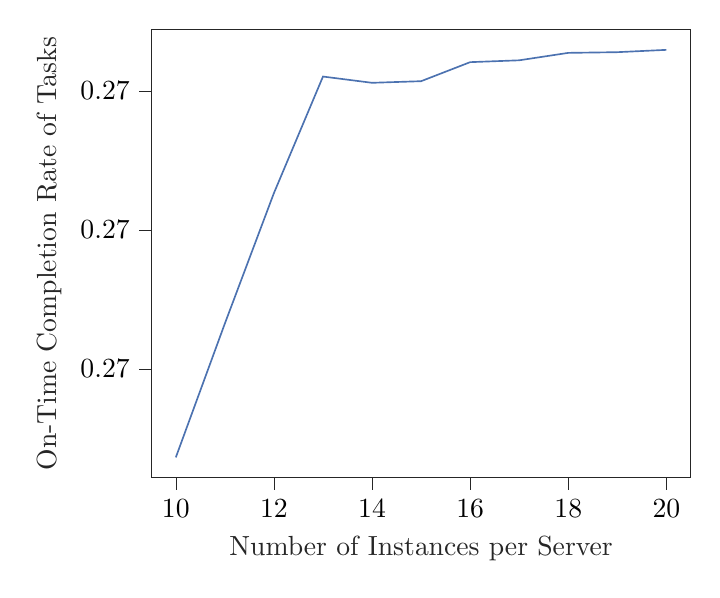
\begin{tikzpicture}

\definecolor{darkslategray38}{RGB}{38,38,38}
\definecolor{lightgray204}{RGB}{204,204,204}
\definecolor{steelblue76114176}{RGB}{76,114,176}

\begin{axis}[
axis line style={darkslategray38},
tick align=outside,
tick pos=left,
x grid style={lightgray204},
xlabel=\textcolor{darkslategray38}{Number of Instances per Server},
xmin=9.5, xmax=20.5,
xtick style={color=darkslategray38},
y grid style={lightgray204},
ylabel=\textcolor{darkslategray38}{On-Time Completion Rate of Tasks},
ymin=0.268435246995995, ymax=0.274882510013351,
ytick style={color=darkslategray38}
]
\addplot [semithick, steelblue76114176]
table {%
10 0.268728304405874
11 0.270654205607477
12 0.272530040053405
13 0.274205607476636
14 0.274115487316422
15 0.274138851802403
16 0.274412550066756
17 0.274439252336449
18 0.27454606141522
19 0.274556074766355
20 0.274589452603471
};
\end{axis}

\end{tikzpicture}
